
\begin{center}
  \begin{tabular}{rl}
  % after \\: \hline or \cline{col1-col2} \cline{col3-col4} ...
  论文地址:& \href{https://arxiv.org/abs/1810.00826}{https://arxiv.org/abs/1810.00826} \\
  源码地址:& \href{https://github.com/weihua916/powerful-gnns}{powerful-gnns} \\
  关键词:& \textbf{GNN, WL graph isomorphism test} \\
  写于:& \date{2020-09-24}
  \end{tabular}
\end{center}

% \par 论文地址:\href{https://arxiv.org/abs/1810.00826}{https://arxiv.org/abs/1810.00826}
% \par GitHub地址:\href{https://github.com/weihua916/powerful-gnns}{powerful-gnns}
% \par 关键词:\textbf{GNN, WL graph isomorphism test}
% \par 写于:\date{2020-09-24}

论文\cite{xu2018how}对以往的GNN模型的表现能力(区分能力)进行了理论上的分析,主要针对不同aggregation 的特点进行了分析,并针对以往的GNNs的弱点,设计了GIN(graph isomorphism network),达到了与WL sub tree相匹配的性能。论文中使用两种分类任务对以往的GNNs和GIN, WL sub tree 进行了测试:结点分类、图分类。

论文由一个问题开始讨论GNNs的区分能力。\\
给定两个图$G_1, G_2$,不同的GNNs可能会将它们(或者两图中的某两个结点)嵌入到相同的表示。这是为什么呢?这就要讨论GNNs是如何来获得结点/图的embeddings了。考虑一个通用的GNN模型:
$$
h_v^{(k)} = COMBINE(h_v^{(k-1)},  AGGREGATE({h_u^{(k-1)} | u \in \mathcal{N}_v } ) )
$$
上式中的$AGGREGATE$用来聚集邻居结点的信息(如mean, max, GRU, LSTM, GAT等),$COMBINE$则用来将聚集后的邻居结点的信息与结点自身的信息进行组合(如拼接。其实这很像一个图中的消息传播模型,现有的很多GNN模型也是基于消息传播的方法来汇聚邻居结点的信息,k层的GNN 相当与汇聚了来自k-hop的邻居的信息。({\color{red}{能否使用其他的框架来构建GNN模型呢?}})对于图$G$的embedding,是由$G$中的所有结点形成的(这涉及graph embedding的问题,参见其他论文)。
$$
h_G = READOUT(h_v^{(K)} | v \in G)
$$
再回到论文中的问题:\textbf{以往的GNN可能无法区分某些结点/图,即对不同的结点/图不能生成唯一的embeddin,不是injective的!}。根据结点/图的embedding生成的方法可以看出,关键在于\\
$AGGREGATE, COMBINE, READOUT$,论文中将这些定义为 \textit{multi-set function},multi-set是一个可以有重复元素的集合,multi-set function就是定义在multi-set上的函数。问题就出在了GNNs使用的某些multi-set function上!
\par 论文主要对不同的AGGREGATE进行了分析,且主要分析了mean, max两种方法。
\begin{figure}[h]
    \centering
    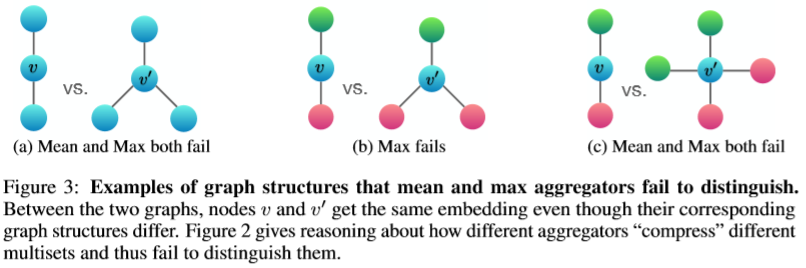
\includegraphics[width=1.\textwidth]{pics/mean-max.png}
    \caption{令Mean, Max失败的例子}
    %\label{fig:my_label}
\end{figure}
如上图所示,展示了mean, max 无法区分两个图中不同结点的邻居情况(neighborhood,即AGGREGATE后的结果是一样的)。论文中分别对mean, max的特性进行了阐述。\\
先给一个形式化的定义,假设$X$为某个结点的邻居结点集,$h(X)$就是AGGREGATE。
\paragraph{MEAN Learns Distributions} 当$h(X) = \frac{1}{|X|}\sum_{x\in X} f(x)$ 时,若对于不同的邻居结点集$X_1, X_2$,若$h(X_1) = h(X_2)$,则$X_1$和$X_2$有着相同的分布。从统计意义上来理解,相当于两个分布的均值(mean)相同。所以,当我们更需要捕捉图中某种信息的分布或者信息重复较少时,mean会有不错的效果。

\paragraph{MAX Identity "Skeleton"}(妙!) 当$h(X) = max_{x\in X}f(x)$时,若对于不同的$X_1, X_2$有$h(X_1) = h(X_2)$,则$X_1$和$X_2$有着相同的underlying set。当使用max作为AGGREGATE时,相当于对multi-set中的“重点”元素进行关注,当放在整个图中看时,相当于抽取了图中某种意义上比较“强”的结点。

\par 接下来就是重头戏 --- GIN了。
\par 论文中对结点和图的GIN定义如下:
$$
h_v^{(k)} = MLP^{(k)} ((1+\epsilon^{(k)} ) \cdot h_v^{(k-1)}+\sum_{u \in \mathcal{N}(v)} h_u^{(k-1)} ))  \newline
$$
$$
h_G = CONCAT(READOUT({h_v^{(k)} | v \in G}) | k = 0,1,...,K)
$$
看到上面的定义,你可能会疑惑,为什么GIN就比其他的GNNs好呢?这和以往的GNNs有什么区别呢?论文中对GIN使用的AGGREGATE进行了理论上的证明,证明GIN是injective的。
\par 论文中通过两个结论证明了GIN的injective性。说了几次injective了,那什么是injective呢?\\
\textbf{injective function}: 定义域中的每个不同的原像在值域中的像都是唯一的。
那么,为了让GNN有足够powerful的表现/识别能力,GNN需要尽可能精确地区分每个不同的结点/图(GNN作为以一种主要的embedding方法,高精度的表示能力能为下游任务打好基础),所以应尽量使AGGREGATE, COMMBINE, READOUT 是injective的。\\
{\color{red}证明GIN的injective}

\par 再来谈一下  Weisfeiler-Lehman (WL) graph isomorphism test 。WL isomorphism test 是用来比较两个图是否是同构的。先解释一下同构的概念。\\
抛开图同构,把同构概念单独拎出来看。对于两个系统中的对象,同构映射能够保持两个系统中的对象一一对应,且对象之间的关系也能够一一对应。图同构中,$v_1 = f(u_1), v_2 = f(u_2),u_1, u_2 \in G_1, v_1, v_2 \in G_2$,若$u_1, u_2$之间有边,则$(v_1, v_2) = g((u_1, u_2))$。\\
WL test 是通过迭代的聚集邻居的标签,每次迭代后将自己的标签和邻居们的标签映射成一个新的标签(相当于AGGREGATE后在COMBINE),迭代完成后比较两个图的标签分布(简单来说即各个标签分别有几个)是否一致({\color{red}结点的标签能否收敛呢?为什么标签的分布能用来判定是否同构呢?}),如果标签分布一致,则两个图可能是同构的。
WL subtree kernel\cite{shervashidze2011weisfeiler} 是基于 WL test的。我并没有通读论文,但是粗略看了一下图,感觉 WL subtree kernel和现在的GNN已经很像了, 对于每个结点,WL subtree kernel构建以该结点为root的树,子节点为其邻居结点,子节点的子节点是邻居结点,如此循环定义,最后以这颗树作为结点标签的依据。WL subtree kernel是目前基于聚合方式的GNNs的性能上界(证明见论文appendix)。但是WL subtree kernel并不能结合结点的信息,对于现在图中结点丰富的信息来说,这不免是有点浪费的,而且,个人认为WL subtree kernel捕捉的是图的结构(毕竟是衍生于图同构算法),或许图中的其他信息它是没有捕捉到的({\color{red}是什么信息呢?}) 

\par 关于未来的研究方向。有没有比基于聚集邻居结点信息(信息传递)方法更好的一个GNN框架呢?

关于WL test可参考的博客/非文献资料:
\begin{enumerate}
    \item \href{https://www.davidbieber.com/post/2019-05-10-weisfeiler-lehman-isomorphism-test/}{The Weisfeiler-Lehman Isomorphism Test}
\end{enumerate}
